\section{Background}

% Brief "what is this?" section to explain structure of background
If we are to visualize accessibility,
a general understanding of research in both accessibility and cartography is necessary.
After briefly presenting both fields,
I will relate the two together
providing a more focused synthesis of the aspects most relevant to this thesis.

\begin{itemize}
	\item Define terms more in depth (cartography, map, accessibility...)
	\item Small history recap of the relevant advances in the field of cartography
	\item Cartographic interaction theory
	\item Web mapping advances and technologies
	\item Interactive accessibility presentations and other relevant maps: go over some previous implementations and solutions.
\end{itemize}

% Cartography - How we got to where we are now, what this means for the topic
\subsection{Cartography and cartographic interaction}

\subsubsection{Defining cartography and maps}
% What cartography?
Depictions of the spatial world
have been present in human communities for thousands of years
(for example \textcite{hsu1993, sch2014}).
However, cartography,
not as in the practice of mapmaking but as in an established science,
is much younger.
In fact, \textcite{woo2003, kai2020} argue that
the discipline of cartography dates back only to the early 1900s,
since that is when a scientific body of theory on maps started to form.
Before that, it was mainly the mathematical theory on map projections
and the production of topographical maps that were associated with cartography \parencite{kai2020}.
In the time that cartography has been considered its own science,
change has been a constant in the discourse within the discipline \parencite{mac2004} --
% the discipline has reinvented itself many times.
cartography is as dynamic as the topics that people map,
or the methods they use to map said topics \parencite{tyn1992, tyn2014}.
Consequently,
the term cartography has been difficult to define \parencite{kry1995},
and even if a definition is agreed upon,
it should be considered a product of the time period
in which it was envisioned \parencite{tyn1992, and1996}.
Currently, the \acrlong{ica} (\acrshort{ica}),
the authoritative international body for cartography,
defines cartography as
\enquote{The science, art, and technology of making and using maps}.
\parencite{ica2019}.

To better understand this definition and,
more importantly, cartography in general,
it is essential to acknowledge the field's multidisciplinary nature.
% Classically, the practice of mapmaking has been associated with art
How a map works is always in some part tied with mathematics.
Representing the curved surface of earth, a geoid in shape,
on a surface of a different shape requires a mathematical transformation.
The effects of this transformation vary by projection, but
regardless of projection, some distortion is always introduced to the map.
For example producing general purpose maps using a projection intended for navigation purposes.
% Formation of the cartography as a discipline

Cartography in its own right comprises many disciplines,
and acts as a tool for many more

\parencite{kai2020}
\textcite{mac2004} considers two developments especially important
to understanding how the modern cartographic research has shaped up.

% 1950
The first, set in motion by the second world war, was
the shift from thinking of maps as primarily objects of art and graphic design,
to instead viewing them as scientifically dissectable visual representations
with the primary function of conveying information.
Interlinked with the field of psychology,
functional map design drew from the research on human perception
in an effort to optimize cartographical methods such as symbology.
The goal of these efforts was finding scientifically provable, "objective", rules
for producing as functional as possible maps.
Cartography does not exist in a vacuum - it is interlinked with other fields of science

% 1970
% Cartography as graphic communication.
The second was the change in how a map is thought to work.
Instead of an artefact of its own knowledge,
a map is essentially just a means to transport knowledge in a communication system.
So, the knowledge a map reader gains from reading a map is that of the mapper's,
just disseminated through cartographical communication, i.e. the map.
Thinking this way, no new knowledge is constructed by the map reader,  % TODO check this & debunk later
and the acts of map making and reading can be related to constructing and interpreting messages.
Draws heavily from the paradigm of graphical communication,  % useless line?
\textcite{bal1966} propose a term, "graphicacy",
to relate the importance of graphical communication to literacy, articulacy and numeracy.
Among the pioneers of this way of thinking about maps was \textcite{kol1969},
who explicitly regarded maps as communication systems.

However, there have been numerous objections to the paradigm of Cartography as a form of communication.
Firstly, there is the issue of communication versus function:
A mapmaker might not have an intent to communicate any particular message to begin with.

Also, implicit vs explicit:
the message the map reader extracts from a map might differ from the one intended, or


% Moving on from these
Art and science \parencite{mac2004, tyn1992}  % compare these

% 1990
% - More interlinked with GIS
% - critical / qualitative GIS too

% 2010-the present -> interactive
% The change in cartography
% Rise of open source \textcite{pet2015}


% What map?
By now it is clear that,
much like cartography,
the concept of a map is anything but static.
In a review of various historical writings \textcite{and1996}
found 321 unique definitions for the word.
Most of these definitions shared the premise that
maps are representations of the surface of the earth,
but, other than that, not many similarities were found.
More current efforts in defining the word range
from lengthy attempts at precise delineation (for example \textcite{ica2003})
to much shorter definitions (for example \textcite{kra2017}).
If the \acrshort{ica} is to be considered an authority, a map is currently
\enquote{an abstract visual representation of the geo-environment} \parencite{ica2019}.

% What map for real?
Even though quite concise,
\acrshort{ica}'s definition has received its fair share of critique as well.
For example, \textcite{lap2021} note that
a map can be a concrete object or have concrete qualities
instead of being strictly abstract,
and be perceived with senses other than vision.
The word \enquote{geo-environment} is problematic too.
It would limit maps to depicting only earth
(an issue found in many map definitions \parencite{tyn2014})
as well as introduce possible confusion with themes such as
environmental sustainability \parencite{lap2021}.
As a response, \textcite{lap2021} suggest that,
instead of a given environment or a type of map,
\textit{spatial relationships} should be the starting point of defining what a map is.
Thus, \citeauthor{lap2021} arrive at the following definition:
\enquote{a map is a generalized representation of spatial relationships}.
A few years earlier, \textcite{tyn2014} shared much of the same sentiments,
defining a map as \enquote{a graphic representation that shows spatial relationships}.
While in her definition \citeauthor{tyn2014} specifies maps as something graphic,
both authors are in agreement that maps are representations,
and that representing spatial relationships is what makes a representation a map.

% Different types of maps

% TODO
% For most of humanitys history maps have been a tool to describe the physical world,
% used for navigation and comprehending places etc
% Nowadays data visualization
% Presenting the world (locations) vs presenting data linked to locations (thematic mapping, \parencite{tyn1992})
% Change, cartography is different now, 1950-1990
\subsubsection{Maps as interfaces}

\parencite{kra2017}
The traditional ‘authoritative’ view of the map being a carefully crafted product
by the cartographer, aimed at visually communicating a complete, mostly static database
of known geographic facts to a user, has turned into a participatory and collaborative perspective.
The map has moved beyond the static window to the world and become an
interactive, mobile, dynamic and collaborative interface between a human, groups of
people and the dynamically evolving environment
% The default medium for viewing maps and geographical has long been digital.  % TODO add ref
% However, more and more devices allow also for interaction \parencite{mei2019}
% \begin{displayquote}


% The nature of interactive cartography
% More than a map: ui, ux
% What even is an interactive cartographer?
% A map is both the for of presentation, as well as the method of interaction
% -> a more complex map means basically a user interface -> need for UI library
\textcite{rot2013a, rot2013b}

\subsection{Crafting interactive map presentations}
\subsubsection{Maps as digital applications}
% What? types of maps & feature scope

\subsubsection{Web maps and mapping technologies}

% Map vs Web gis

% technologies

\subsection{Cartographic presentation of accessibility}

\subsubsection{Accessibility as a phenomenon}
% Difficulty & potential for interaction

Alone, the word accessibility simply refers to how easy it is to access something,
with all further meaning derived from
additional explanations and the context in which the word is used.
Maybe history? Background \parencite{ten2020}

Components: people, transport, activities \parencite{jar2018}

% What makes accessibility a unique phenomenon,


% The previous but from a cartographical point of view.
% What requirements this places on visual representations of accessibility.

\subsubsection{Approaches in visualizing accessibility}

% Interactivity in general
% What value do interactive visualizations hold in the context of accessibility?
% (General theory of cartography and especially cartographic interaction,
% previous interactive maps and presentations relative to the topic.)
% \end{displayquote}

% Here I will be doing literature review as well,
% especially relating to the theory of cartography and interactive maps.
% Themes such as critical cartography
% and the qualitative nature of maps should be found here too.
% When previewing previous accessibility visualizations,
% some kind of systematic comparison of previous work
% could be a way to form a synthesis here.

\begin{figure}[H]
	\centering
	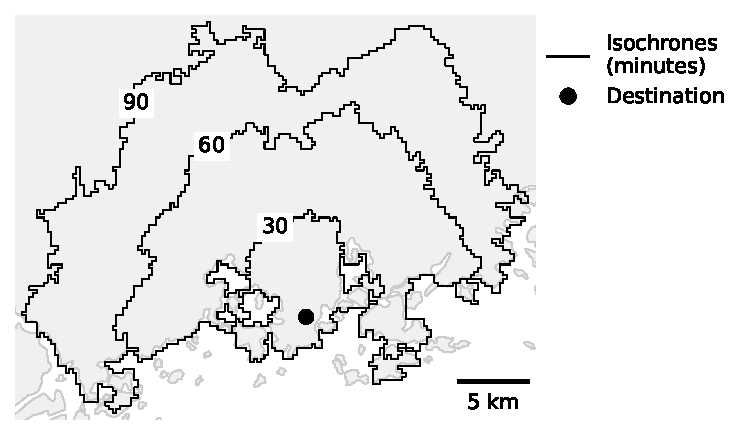
\includegraphics[width=0.6\textwidth]{visual/figures/ttm/isochrone_lines.pdf}
	\caption{Isochrones}
	\label{fig:isochrone lines}
\end{figure}

\begin{figure}[H]
	\centering
	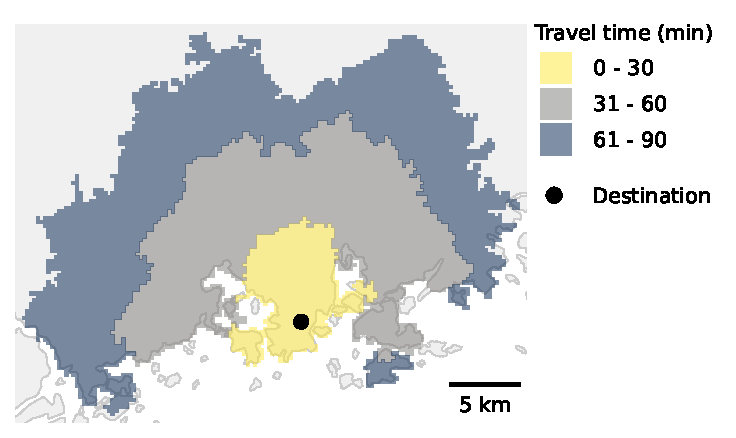
\includegraphics[width=0.6\textwidth]{visual/figures/ttm/isochrone_areas.pdf}
	\caption{Areas between isochrones}
	\label{fig:isochrone areas}
\end{figure}

% TODO
% Mention tradeoffs (detail - speed) -> leads to methods
Crafting any cartographical presentation is much about tradeoffs.
Often these tradeoffs are concerned with the visual composition of the presentation --
what the map can and should try to communicate.

% TODO
Previous presentations can be very precise, but locked to a single place

